\documentclass[a4paper,10pt]{book}

\usepackage{listings}
\usepackage{graphicx}
\usepackage{color}
\usepackage{bm}
\usepackage{amsmath}
\usepackage{appendix}
\usepackage{xspace}
\usepackage{a4wide}
\usepackage{hyperref}

\renewcommand{\vec}[1]{\ensuremath{{\bm #1}}}
\newcommand{\fig}[1]{fig.~\ref{#1}}
\newcommand{\eq}[1]{eq.~\ref{#1}}
\newcommand{\unit}[1]{\ensuremath{\,\mbox{#1}}}
\newcommand{\ibi}{IBI\xspace}
\newcommand{\imc}{IMC\xspace}
\newcommand{\fm}{FM\xspace}
\newcommand{\xml}{XML\xspace}
\newcommand{\gromacs}{GROMACS\xspace}
\newcommand{\spce}{SPC/E\xspace}
\newcommand{\grad}{\vec{\nabla}}
\newcommand{\ddash}{{-}{-}\xspace}
\newcommand{\csgfmatch}{\textbf{csg\_fmatch}\xspace}

\newcommand{\sect}[1]{sec.~\ref{#1}}

\newcommand{\votca}{{\sc votca}\xspace}

\newcommand{\sasha}{ {\sc \color{red} Alexander Lukyanov} \newline}
\newcommand{\denis}{ {\sc \color{red} Denis Andrienko} \newline}

\begin{document}
\pagenumbering{roman}
\begin{titlepage}
  \title{VOTCA - User Manual}
  \author{Victor R\"uhle, Christoph Junghans, Alexander Lukyanov, Kurt Kremer, Denis Andrienko}
  \maketitle
\end{titlepage}
\newpage 
\thispagestyle{empty}
\quad 
\newpage

\thispagestyle{empty}
\tableofcontents
\newpage
\quad 
\newpage

\setcounter{page}{1}
\pagenumbering{arabic}

\chapter{Introduction}
\label{sec:introduction}

Charge carrier dynamics in an organic semiconductor can often be described in terms of charge hopping between localized states. The hopping rates depend on electronic coupling elements, reorganization energies, and driving forces, which vary as a function of position and orientation of the molecules.  The exact evaluation of these contributions in a molecular assembly is computationally prohibitive. Various, often semi-empirical, approximations are employed instead. The purpose of \votcactp is to simplify the workflow for charge transport simulations, provide a uniform error-control for the methods, flexible platform for their development, and eventually allow in silico pre-screening of organic semiconductors for specific applications. 

The toolkit is implemented using modular concepts introduced earlier in the Versatile Object-oriented Toolkit for Coarse-graining Applications (VOTCA)~\cite{ruehle_versatile_2009}. The VOTCA structures are adapted to reading atomistic trajectories, mapping them onto conjugated segments and rigid fragments, and substituting (if needed) rigid fragments with the optimized copies. 

The \hyperref[sec:moo]{molecular orbital overlap} module calculates electronic coupling elements between  conjugated segments from the corresponding molecular orbitals. It relies on the semi-empirical INDO Hamiltonian and molecular orbitals in the format provided by the \gaussian package. An alternative,  \hyperref[sec:dft]{density-functional based approach}, has interfaces to the \gaussian and \turbomole packages. An interface to the \tinker package is provided for calculations of electrostatic and polarization contributions to energetic disorder. 

The  \hyperref[sec:kmc]{kinetic Monte Carlo module} reads in the neighbor list, site coordinates, and hopping rates and performs charge dynamics simulations using either periodic boundary conditions or charge sources and sinks. 

The toolkit is written as a combination of modular C++ code and scripts. The data transfer between programs is implemented via a state file or database, which is also used to restart simulations. Analysis functions and most of the calculation routines are encapsulated by using the observer pattern~\cite{gamma_design_1995} which allows the implementation of new functions as individual modules.
\chapter{Theoretical background}
\label{sec:theory}

\section{Workflow}
A typical workflow of charge transport simulations is depicted in \fig{workflow}. The first step is the simulation of an \hyperref[sec:morphology]{atomistic morphology}, which is then partitioned on \hyperref[sec:mapping]{hopping sites}. The coordinates of the hopping sites are used to construct a list of pairs of molecules (neighbor list). 

\begin{figure}[h]
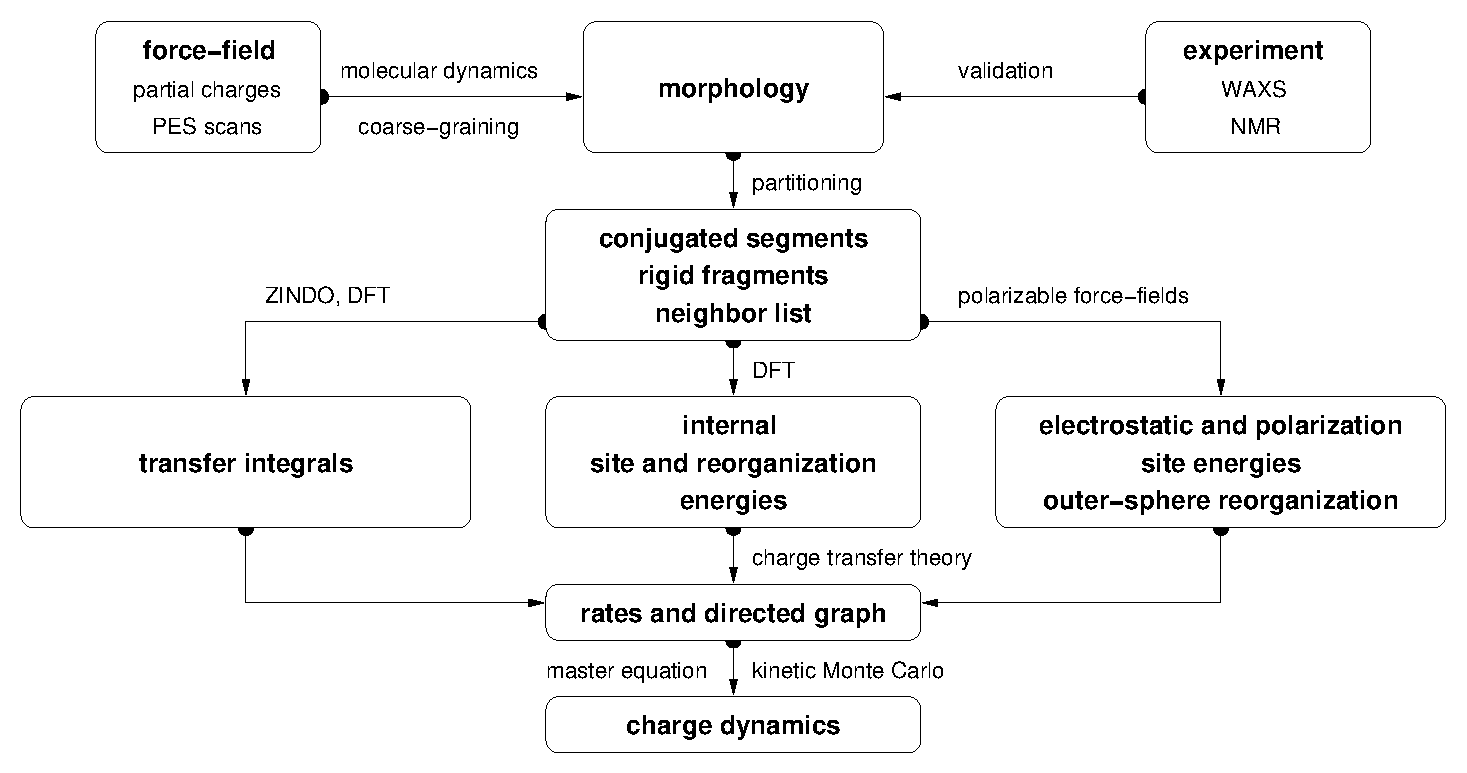
\includegraphics[width=\textwidth]{fig/workflow/workflow}
 \caption{%
   Workflow for microscopic simulations of charge transport.  %
   \label{fig:workflow}}
\end{figure}

For each pair an \hyperref[sec:transfer_integrals]{electronic coupling element}, a reorganization energy, a driving force, and eventually the hopping rate are evaluated. The neighbor list and hopping rates define a directed graph. The corresponding master equation is solved using the  \hyperref[sec:kmc]{kinetic Monte Carlo method}, which allows to explicitly monitor the charge dynamics in the system as well as to calculate time- or ensemble averages of occupation probabilities, charge fluxes, correlation functions, and field-dependent mobilities.


\section{Conjugated segments and rigid fragments}
\label{sec:conjugated_segments}

With the morphology at hand, the next step is partitioning the system on hopping sites, or conjugated segments, and calculating charge transfer rates between them. Physically intuitive arguments can be used for the partitioning,  which reflects the localization of the wave function of a charge. For most organic semiconductors, the molecular architecture includes relatively rigid, planar $\pi$-conjugated systems, which we will refer to as rigid fragments. A conjugated segment can contain one or more of such rigid fragments, which are linked by bonded degrees of freedom. The dynamics of these degrees of freedom evolves on timescales much slower than the frequency of the internal promoting mode. In some cases, e.g. glasses, it can be `frozen' due to non-bonded interactions with the surrounding molecules.

\begin{wrapfigure}{ht}{0.5\linewidth}
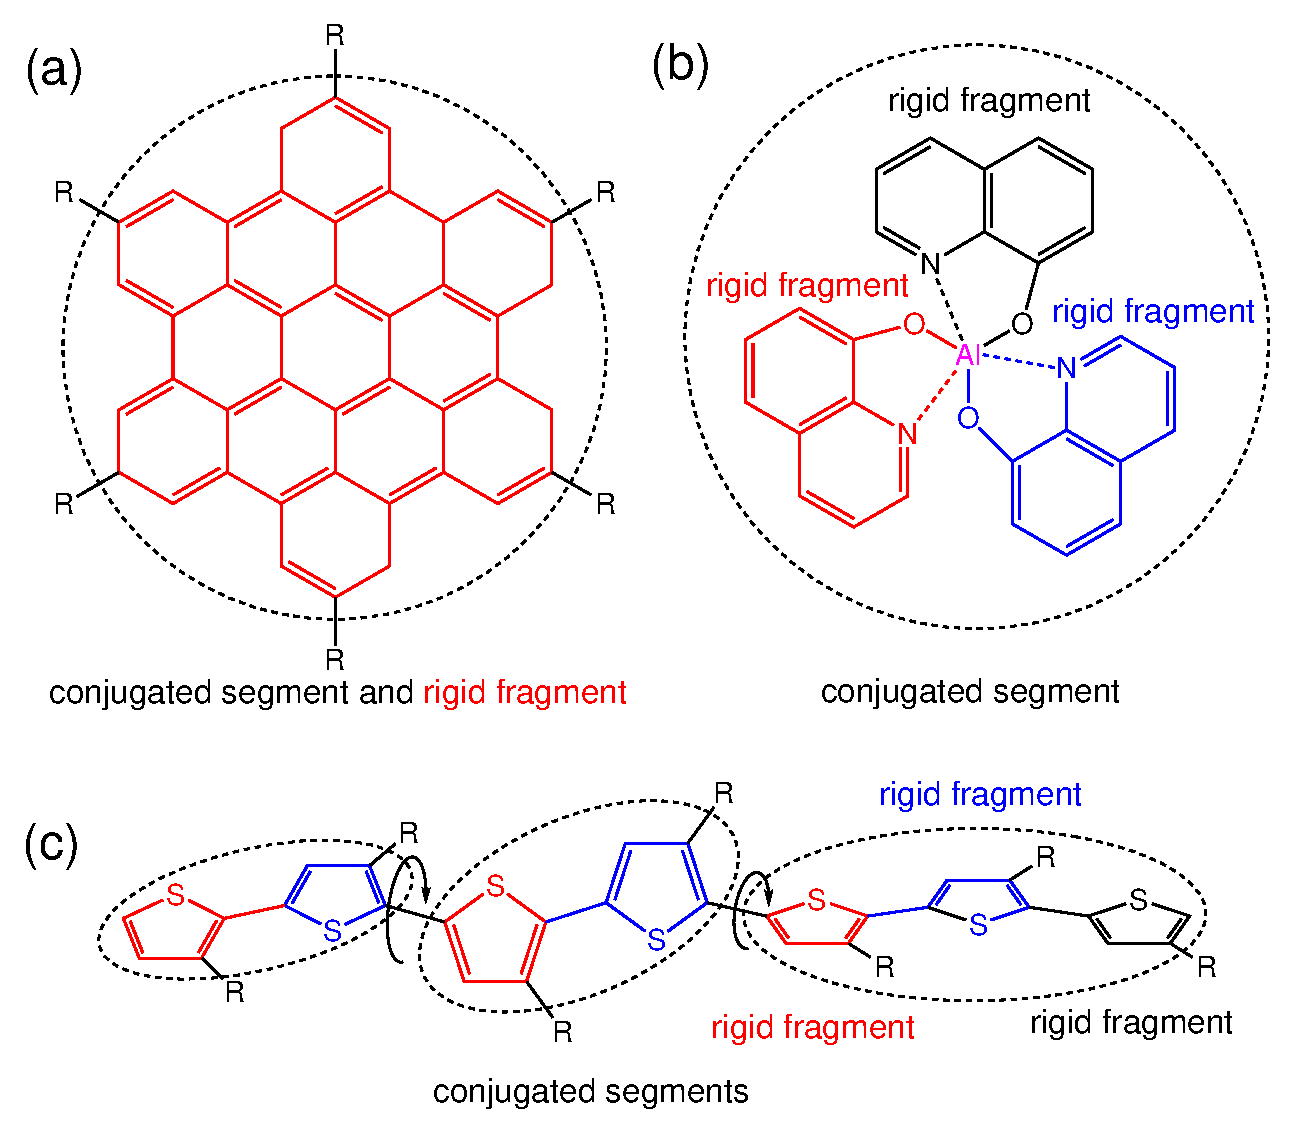
\includegraphics[width=\linewidth]{fig/conjugated_segment/fragment_segment}
\caption{\small The concept of conjugated segments and rigid fragments. Dashed lines indicate conjugated segments while colors denote rigid fragments. (a) Hexabenzocoronene: the $\pi$-conjugated system is both a rigid fragment and a conjugated segment. (b) \Alq: the Al atom and each ligand are rigid fragments while the whole molecule is a conjugated segment. (c) Polythiophene: each repeat unit is a rigid fragment. A conjugated segment consists of one or more rigid fragments. One molecule can have several conjugated segments.}
\label{fig:segment}
\end{wrapfigure}


To illustrate the concept of conjugated segments and rigid fragments, three representative molecular architectures are shown in \fig{segment}. The first one is a typical discotic liquid crystal, hexabenzocoronene. It consists of a conjugated core to which side chains are attached to aid self-assembly and solution processing. In this case the orbitals localized on side chains do not participate in charge transport and the conjugated $\pi$-system is both, a rigid fragment and a conjugated segment. 
%
In \Alq, a metal-coordinated compound, a charge carrier is delocalized over all three ligands. Hence, the whole molecule is one conjugated segment. Individual ligands are relatively rigid, while energies of the order of $k_\text{B}T$ are sufficient to reorient them with respect to each other. Thus the Al atom and the three ligands are rigid fragments.
%
In the case of a conjugated polymer, one molecule can consist of several conjugated segments, while each backbone repeat unit is a rigid fragment. Since the conjugation along the backbone can be broken due to large out-of-plane twists between two repeat units, an empirical criterion, based on the dihedral angle, can be used to partition the backbone on conjugated segments~\cite{ruehle_multiscale_2010}. However, such intuitive partitioning is, to some extent, arbitrary and shall be validated by other methods~\cite{vukmirovi_charge_2008,vukmirovi_charge_2009,mcmahon_ad_2009}. 

After partitioning, an additional step is often required to remove bond length fluctuations introduced by molecular dynamics simulations, since they are already integrated out in the derivation of the rate expression. This is achieved by substituting respective molecular fragments with  rigid, planar $\pi$-systems optimized using first-principles methods. Centers of mass and gyration tensors are used to align rigid fragments, though a custom definition of local axes is also possible. Such a procedure also minimizes discrepancies between the force-field and first-principles-based ground state geometries of conjugated segments, which might be important for calculations of electronic couplings, reorganization energies, and intramolecular driving forces. 

Finally, a list of neighboring conjugated segments is constructed. Two segments are added to this list if the distance between centers of mass of {\em any} their rigid fragments is below a certain cutoff. This allows neighbors to be selected on a criterion of minimum distance of approach rather than center of mass distance, which is useful for molecules with anisotropic shapes.

\chapter{Implementation}
\subsection{Coarse-graining engine}
\votca can be divided into two main parts. A C++ kernel, which includes various coarse-graining tools and is capable of processing topologies and trajectories, and a scripting enginge to steers the iterative procedures.

These tools include calculations of probability distributions of bonded and non-bonded interactions, correlation and autocorrelation functions, and updates for the coarse-grained pair potential. Analysis tools of the MD package can also be integrated into the coarse-graining workflow, as needed.

The package offers a flexible framework for reading, manipulating and analyzing of MD/SD/MC topologies and trajectories. Its core is modular and new file formats can be integrated without changing the existing code. Currently, an interface for \gromacs~\cite{gromacs4} topologies and trajectories is provided.

The coarse-graining procedure itself is controlled by several Extensible Markup Language (\xml) input files, which contain mapping and other options required for the workflow control. For the mapping, it is possible to select groups of interactions which are used for the coarse-graininged analysis. 
%It is possible to generate exclusion lists for Boltzmann inversion of bonded interactions or virtual sites for back-mapping.

\section{Mapping definitions}
{\em Mapping definitions} describe how to map a single molecule from atomistic to coarse-grained representation. The mapping definition have only to be specified once per molecule. The file contains sections for coarse-grained beads, bonded interactions in coarse grained scheme as well as mapping matrices. 

\subsection{Example - mapping file for propane}

\lstinputlisting[frame=single,caption=Mapping for propane]{functionality/propane.xml}


\section{Topologies}
A topology is defined as a set of beads with a certain bead type which are connected by bonded interactions.
Votca can read topologies in the \gromacs tpr format. Additionally, it can use a pdb file as topology, however, not all information are given in a pdb file and are not defined. If a pdb topology is used, it is recommended to fill additional molecule information using the xml advanced topology handling feature (see. \sect{sec:adv_topology})
\subsection{Manual topology handling}
\label{sec:adv_topology}
Many file formats do not have a clear definition of a molecules. This can lead to problems, especially if a simulation contains several multiple molecules. Since during the coarse graining, the molecule type is identified by a name tag, names must be set properly. \votca offers the possibility to read a topology and later on modify parts of it. Everything is defined in an xml topology file.

Also \gromacs did not store molecule names in previous versions. This was introduced in a newer release. If possible, always provide a recent .tpr file which contains molecule names. For old topologies, rerun grompp if possible to get a recent file.

If a system with multiple molecule types is processed, but no molecule names are present, molecule names have to be specified manually as described in this section that \votca can choose the correct mapping scheme..

If no molecule information is present at all, they can be created. An for a topology file that reads in last.pdb and then creates molecules is:
\begin{lstlisting}
<topology base="last.pdb">
  <molecules>
    <clear/>
    <define name="mCP" first="1" nbeads="52" nmols="216"/>
  </molecules>
</topology>
\end{lstlisting}
<clear/> clears all bolecule information that were present before.

If the file format the topology is read from only does not support molecules names, \votca offers the possibility to define topologies in an xml file and manipulate the molecule names after reading. A short example:
\begin{lstlisting}
 <topology base="topol.tpr">
   <molecules>
     <rename name="PPY3" range="1:125"/>
     <rename name="Cl" range="126:250"/>
   </molecules>
 </topology>
\end{lstlisting}
Here, first to file topol.tpr is loaded. The file supports molecules but does not give a name tag. Afterwards, Molecules are renamed. This file can be loaded as any other topology.

To use the new topology, create a file using the schema above and save it as .xml. To use it in the program, you'll have to give several coarse graining definitions, separated by ;. If you saved the example above as newtop.xml, use 

\subsection{Trajectories}
A trajectory is defined as a set of frames containing coordinates and eventually velecities and forces for the beads of a topology.
VOTCA currently supports trr, xtc, pdb and gro as trajector formats.

\section{Iterative workflow control}
\label{sec:impl:scripting}
For each iterative method (e.g. IBI or IMC), a simulation has to be performed with a working potential. Based on statistics from that coarse grained run, an update can be calculated. \votca implements a flexible scripting framework to perform such an iterative workflow. The workflow chart is shown in \fig{fig:flowchart}. The workflow is implemented as a shell script which can, in principle, be run on all available operating systems and provides the flexibility needed to call external (or overload existing) scripts and programs written in other programming languages. An interface to read values from the steering \xml files in C++, Perl and shell is also provided.

\begin{figure}
  \includegraphics[width=0.7\columnwidth]{functionality/fig/flowchart.eps}
  \caption{
    \label{fig:flowchart}
    Block-scheme of the workflow control for the iterative methods. The most time-consuming parts are marked in red.
  }
\end{figure}

During the global initialization the initial guess for the coarse-grained potential is calculated from the reference radial distribution function or converted from a given potential guess to the internal format. The actual iterative step starts with an iteration initialization. It searches for possible checkpoints and copies and converts files from the previous step and the base directory. Then the simulation run is prepared by converting potentials to the format required by the external sampling program and actual sampling is performed. Currently, an interface with \gromacs~\cite{gromacs4} is implemented and extension to other packages is straightforward. After sampling the phasespace, potential update $\Delta U$ is calculated. Often the update requires postprocessing, such as smoothing, interpolation, extrapolation or fitting to an analytical form. A simple pressure correction~\cite{Reith:2003} can also be seen as a postprocessing of $\Delta U$, due to the fact that it only adds a linear interparticle separation function.
%
Finally, the new potential is determined and postprocessed. If the iterative process continues, the next iterative step starts to initialize.

\subsection{General usage}
To setup the environment, run:
csh, tcsh:
\begin{verbatim}
  source <csg-installation>/bin/CSGRC.csh
\end{verbatim}
\begin{verbatim}
  bash: source <csg-installation>/bin/CSGRC.bash
\end{verbatim}

Tutorials can be found in \textit{$<$csg-installation$>$/share/csg/tutor}. Just copy one of the tutorial and try
\begin{verbatim}
 csg_inverse <options.xml>
\end{verbatim}

\subsection{Run preparation}
To run the iterations, the input for the sampling program (e.g. \gromacs ) has to be prepared in order to carry out one iteration. All files for running a coarse-grained simulation except for the tabulated potentials that should be created must be present and specified in the options xml-file.

As target distribution, any table file can be given (e.g. gromacs output from g\_rdf). The program automaticaly takes care to resample the table to the correct grid spacing as specified in the .xml file.
The initial guess is created by inverting the rdf. It's located in step\_00/$<$name$>$.pot.new. To specify the initial guess for a specific interaction by hand, write the potential table to a file called $<$name$>$.pot.in in the folder where you run the iterative procedure.

To define which interactions are iteratively refined, a section for each has to be specified in the config file. A full list of parameters can be found in ref.~\ref{sec:ref_options}.

\subsection{Running the iterative process}
After all input is set up, the run can be started with
\begin{verbatim}
  csg_inverse <options.xml>
\end{verbatim}

For each iteration, a separate folder (\textit{step\_$<$iteration$>$}) is created, where \textit{step\_00} has the special meaning of the initial setup before the first iterations. For each new iterations, the files required to run the CG simulation ( as specified in the config file) are copied to the current working folder. Also the updated potentials from the last steps ( stetp\_$<$n-1$>$/$<$interaction$>$.pot.new ) are copied and used as the new working potentials ( stetp\_$<$n$>$\/$<$interaction$>$.pot.cur ).

After the preparation, the simulation run is started. First, all potentials are converted to the format of the sampling program, and the simulation is started. As soon as the run is finished, analysis programs are started and new distributions calculated ( $<$interaction$>$.dist.new ) and the update is calculated ( $<$interaction$>$.dpot.new ). Before \votca adds the update to the old potential, the update can be processed in the post\_update step. For each script that is specified in post\_update, \votca renames $<$interaction$>$.dpot.new to $<$interaction$>$.dpot.old, stores it in $<$interaction$>$.dpot.$<$a-number$>$, and calls the processing script. Each processing script us supposed tok takes the current update ( $<$interaction$>$.dpot.cur ) and write the processed update to ( $<$interaction$>$.dpot.new ). As described, \votca takes care for all the renaming. Pressure correction is implemented as a post\_update script within this framework.

After all post\_update scripts are called, the update is added to the potential and the new potential ( $<$interaction$>$.pot.new ) is written. After that, processing of the potential is performed in the post\_add step, analogous to the tasks performed in post\_update but now for the potential instead of the update.

As a summary, the standard output files of \votca for each step are listed in the following table:

\begin{tabular}{ll}
*.dist.new & distribution functions of the current step \\
*.dpot.new & the final potential update, created in calc\_update \\
*.dpot.$<$number$>$ & for each post\_update script, the current .dpot.new is saved and a new one is created\\
*.pot.cur & the current potential, the actual run was performed with \\
*.pot.new & the new potential after add step \\
*.pot.$<$number$>$ & same as dpot.$<$number$>$ just for post\_add
\end{tabular}

If some sub step within one iteration failed, additional information can be found in the log file. The name of the log file is specified in the options xml-file.

\subsection{Continue a run}
There are two scenarios when one wants to continue a run: A finished run should be extended or the run was interrupted and one needs to restart at the current point. When csg\_inverse is started, it automatically checks for a file called \textit{done} ine the current folder. If that exists, it assumes the run as done. To extend the run, increase max\_iterations in the settings file and remove the file called done. After that, csg\_inverse can be just restarted, it will recognize available steps and continues after the last one.

If a run was interrupted, csg\_inverse might not be able to restart on it's own. In that case, the easiest solution is to delete the last step and just start again. This will just redo the last step and continue. However this method is not always practical since sampling + analysis might take very long and the run just crashed due to some post processing option. To avoid redoing the whole run, VOTCA creates a file with restart points, that marks actions in the step which were already completed (like simulation, analysis, ...). The file is specified in the option \textit{restart\_????}. If specific actions should be redone, lines in that files can also removed by hand. In addition, a file \textit{done} is created int each folder for a step that already has finished.

\subsection{Customization}
\textbf{Customization of the iterative process it not well documented yet. Documentation will improve in the near future, feel free to ask on the votca mailing list for details! }

In principle, each sub step of an iteration can be changed. All scripts that are called can be redirected ( overloaded ) to user scripts. Please never ever change the \votca installation scripts. Better copy the script and redirect it's call.

The file $<$csg-install$>$/share/csg/scripts/inverse/csg\_table assigns to two given keywords a script which is called. You can change this by creating a file
csg\_table in your own directory ( specified in the Coarse graining directives ). Just add a line for each script you want to add or change. The source\_wrapper takes care that your script is called instead of the one from the standard installations. For scripting details have a look at the source, there is no developers manual so far.






\chapter{Boltzmann Inversion}
\begin{figure}
   \centering
   \includegraphics{usage/fig/flow_boltzmann.eps}
   \caption{Flowchart to perform Boltzmann inversion.}
\end{figure}

Boltzmann inversion is most often performed on a single molecule in vacuum for deriving bonded interactions while the non-bonded parts are treated via a separate method. VOTCA offers tools to analyze distributions and correlations of such a simulation as well as the preparation of a tabulated potential. Also, when the separation ansatz\cite{Tschoep:1998} is used, exclusion lists for the atomistic simulations can be created automatically. The tool most often used in this section is \prog{csg_boltzmann}. In addition,  mapping from the atomistic to the coarse-grained level can be performed using \prog{csg_map}. An important thing to remember when using \prog{csg_boltzmann} is that it parses the whole trajectory and stores all information about bonded interactions in memory, allowing interactive analysis. Hence it is not suitable for really big systems with lots of chains. If analysis of a big system is performed, \prog{csg_stat} should be preferred for the analysis. Although it currently offers less features than \prog{csg_boltzmann}, memory problems should not occur.

\section{Mapping scheme}
The first thing to coarse-grain a system is to define a mapping scheme (see \sect{sec:mapping}). The mapping is defined by a simple xml file for each molecule-type. An important step is to verify the mapping scheme by:

\begin{verbatim}
  csg_map --top topol.tpr --trj traj.trr --cg mapping.xml --out cg.gro
\end{verbatim}

Make sure that the \mapopt{ident} tag matches the molecule name in the reference system. One of the most common things that can go wrong is that beads cannot be found due to wrong naming. To debug which atoms are read in from a topology file, \prog{csg_dump} can be used. A second reason could be, that molecules are not identified correctly for the case of a multicomponent system. See \sect{sec:adv_topology} for details.

In case everything works as desired, a file cg.gro is created which contains the coarse-grained trajectory. An easy way to compare coarse-grained and atomistic representations is to open both in a visualization program (e.g. vmd).  In vmd, be careful when e.g. opening a .gro and .trr file. In this case, the first frame is read from the .gro and all of the following from the .trr. The coarse-grained file only contains the frames from the trajectory, thus in order to compare the trajectories, the first frame of the atomistic run has to be deleted!!

\section{Generating reference trajectories with proper exclusions}
When the Boltzmann inversion method was described in Ref.\cite{Tschoep:1998}, bonded and non-bonded interactions were treated separately. To do this, a special atomistic trajectory is needed, where all non-bonded interactions are excluded which do not contribute to a bonded interaction in the coarse-grained model. Manually, this can be a complicated task, but \prog{csg_boltzmann} offers the option \progopt{--excl} to do this automatically.

To generate an exclusion list, an atomistic topology without exclusions and a mapping scheme has to be prepared first. Since \votca can currently only read GROMACS .tpr trajectories and not .top files, running \progex{grompp} is obligatory. Important to note here is, that \prog{csg_boltzmann} currently only creates the exclusion list for the fist mulecule in the topology.

To create the exclusion list, run
\begin{verbatim}
  csg_boltzmann --top topol.tpr --cg mapping.xml --excl exclusions.txt
\end{verbatim}
This will create a list of exclusions for all interactions that are not within a bonded interaction of the coarse-grained sub-bead. As an example consider coarse-graining of a linear chain of three beads  which are only connected by bonds. In this case, \prog{csg_boltzmann} will create exclusions for all non-bonded interactions of atoms in the first bead with atoms of the 3rd bead as these would contribute only to the non-bonded interaction potential which is treated separately.

To add the exclusions to the \gromacs topology of the molecule, either include the file specified in --excl as follows
\begin{verbatim}
  [ exclusions ]
  #include "exclusions.txt"
\end{verbatim}
or copy and paste the content of that file to the exclusions section.


\section{Analysis}
If the \progopt{--trj} option is specified to parse a reference trajectory, \prog{csg_boltzmann} enters an interactive mode which accepts commands. Here, analysis operations can be performed on all interactions evaluated.

\begin{verbatim}
  csg_boltzmann --top topol.top --trj traj.trr --cg mapping.xml
\end{verbatim}

The interactive mode contains a built in \textit{help} command. To get help on a specific command use
\begin{verbatim}
  help <command>
\end{verbatim}
for example
\begin{verbatim}
  help hist
  help hist set periodic
\end{verbatim}

All interactions specified in the mapping scheme are evaluated. A specific interaction is referred to by a name which is composed of \textit{molecule:interaction-group:index}, where molecule is the molecule number in the whole topology, interaction-group the name specified in the mapping file, and index the entry in the list of interactions. E.g. \textit{1:AA-bond:10} is the 10th AA-bond in molecule 1. To show a list of all interactions that where passed, the command \textit{list} can be used. To specify a couple of interactions during analysis, either give interactions separated by space or use wildcards (e.g. *:AA-bond*).

To exit the interactive mode, use the command \textit{q}. If analysis commands are t be read from a file, use the pipe or stdin redirects from the shell.
\begin{verbatim}
  cat commands | csg_boltzmann topol.top --trj traj.trr --cg mapping.xml
\end{verbatim}

\subsection{Distribution functions and tabulated potentials}
Distribution functions (tabulated potentials) can be created with the \textit{hist} (\textit{tab}) command.
E.g. to write out the distribution function for all interactions of group AA-bond (where AA-bond is the name specified in the mapping scheme) to the file AA.txt, type
\begin{verbatim}
  hist AA.txt *:AA-bond:*
\end{verbatim}
The command
\begin{verbatim}
  hist set
\end{verbatim}
prints a list of all parameters that can be changed for the histogram. To directly write the Boltzmann-inverted potential, the \textit{tab} command can be used. Its usage and options are very similar to the \textit{hist} command. If tabulated potentials are written, special care should be taken to the parameters \textit{T} (temperature) and the \textit{scale}. The \textit{scale} enables volume normalization as given in \eq{eq:boltzmann_norm}. Possible values are \textit{no} (no scaling), \textit{bond} (normalize for bonds) and \textit{angle} (normalize for angles). E.g. to write out the tabulated potential for an angle potential where the temperature is 300K type:
\begin{verbatim}
  tab set T 300
  tab set scale angle
  tab angle.pot *:angle:*
\end{verbatim}

\subsection{Correlation analysis}
\prog{csg_boltzmann} offers two possibilities to evaluate correlations of interactions. On thing is the linear correlation coefficient using the command \textit{cor}. However this is not a good measure since it only calculates the linear correlation and often give misleading results~\cite{Ruehle:2009.a}. A better way is to create 2D Histograms. This can be performed by writing out the values (e.g. bond length, angle, dihedral value) using the command \textit{vals}, e.g.:
\begin{verbatim}
  vals vals.txt 1:AA-bond:1 1:AAA-angle:A
\end{verbatim}
This will create a file which contains 3 columns, the first being the time, and the second and third the bond and angle, respectively. Columns 2 and 3 can either be used to generate the 2D Histogram, or a simpler plot of column 3 over 2, whose density of points reflect the probability.

\chapter{Force matching}
\begin{figure}
   \centering
   \includegraphics{usage/fig/flow_fmatch.eps}
   \caption{Flowchart to perform force matching.}
\end{figure}
The force matching algorithm with cubic spline basis is implemented in the \prog{csg_fmatch} utility. A list of available options can be found in the reference section of \prog{csg_fmatch} (command \texttt{--h}).

\section{Program input}
\prog{csg_fmatch} needs an atomistic reference run to perform coarse-graining. Therefore, the trajectory file {\em must contain forces } (note that there is a suitable option in the \gromacs ~.mdp file), otherwise \prog{csg_fmatch} will not be able run.

In addition, a mapping scheme has to be created, which defines the coarse-grained model (see \sect{sec:mapping}). At last, a control file has to be created, which contains all the information for coarse-graining the interactions and parameters for the force-matching run. This file is specified by the tag \progopt{--options} in the \xml format. An example might look like the following
\begin{lstlisting}
   <cg>
     <!--fmatch section -->
     <fmatch>
       <!--Number of frames for block averaging -->
       <frames_per_block>6</frames_per_block>
       <!--Constrained least squares?-->
       <constrainedLS>false</constrainedLS>
     </fmatch>
     <!-- example for a non-bonded interaction entry -->
     <non-bonded>
       <!-- name of the interaction -->
       <name>CG-CG</name>
       <type1>A</type1>
       <type2>A</type2>
       <!-- fmatch specific stuff -->
       <fmatch>
         <min>0.27</min>
         <max>1.2</max>
         <step>0.02</step>
         <out_step>0.005</out_step>
       </fmatch>
     </non-bonded>
   </cg>
\end{lstlisting}
A full description of all available options can be found in \sect{sec:ref_options}.

\section{Program output}
\prog{csg_fmatch} produces a separate .force file for each interaction, specified in the CG-options file (option \progopt{options}).
These files have 4 columns containing distance, corresponding force, a table flag and the force error, which is estimated via a block-averaging procedure.
If you are working with an angle, then the first column will contain the corresponding angle in radians.

To get table-files for \gromacs, integrate the forces in order to get potentials and do extrapolation and potentially smoothing afterwards.

Output files are not only produced at the end of the program execution, but also after every successful processing of each block. The user is free to have a look at the output files and decide to stop \prog{csg_fmatch}, provided the force error is small enough.

\section{Integration and extrapolation of .force files }
To convert forces (*.force) to potentials (*.pot), tables have to be integrated. To use the built-in integration command from the scripting framework, execute
\begin{verbatim}
 csg_call table integrate CG-CG.force CG-CG.pot
\end{verbatim}

This command calls the \prog{integrate.pl} script, which integrates the force and writes the potential to the .pot file.

In general, each potential contains regions which are not sampled. However, a special value can be defined in the tabulated potential file for the simulation program. This can be used to never sample very small distances in the case of non-bonded interactions or to extend the file to long ranges. To extrapolate the potential, the grid has to be resampled first as shown below
\begin{verbatim}
 csg_resample --in CH2-CH2.pot --out CH2-CH2.resampled.pot --grid 0:0.001:1.4
\end{verbatim}

Finally, the \prog{extrapolate.pl} script can be called:
\begin{verbatim}
 csg_call table extrapolate --function linear
--region leftright CH2-CH2.resampled.pot CH2-CH2.extrapolated.pot
\end{verbatim}

\chapter{Iterative methods}
\label{sec:iterative_methods}

The following sections deal with the methods of Iterative Boltzmann Inversion
(\ibi), Inverse Monte Carlo (\imc), and Relative Entropy (\re).

In general, \ibi, \imc, and \re are implemented within the same
framework. Therefore, most settings and parameters of those methods are similar
and thus described in a general section (see
sec. \ref{sec:iterative_methods_imc}). Further information on iterative methods
follows in the next chapters, in particular on the \ibi, \imc, and \re methods.

\begin{figure}[h]
   \centering
   \includegraphics[width=7cm]{usage/fig/flow_ibi.eps}
   \caption{\label{fig:flow_ibi}Flowchart to perform iterative Boltzmann inversion.}
\end{figure}

\section{Iterative workflow control}
\label{sec:iterative_workflow}

\begin{figure}[t]
   \centering
   \includegraphics[width=7cm]{functionality/fig/flowchart.eps}
   \caption{\label{fig:flowchart}Block-scheme of the workflow control for the iterative methods. The most time-consuming parts are marked in red.}
\end{figure}

Iterative workflow control is essential for the \ibi, \imc, and \re methods.

The general idea of iterative workflow is sketched in fig.~\ref{fig:flowchart}. During the global initialization the initial guess for the coarse-grained potential is calculated from the reference function or converted from a given potential guess into the internal format. The actual iterative step starts with an iteration initialization. It searches for possible checkpoints and copies and converts files from the previous step and the base directory. Then, the simulation run is prepared by converting potentials into the format required by the external sampling program and the actual sampling is performed.

After sampling the phasespace, the potential update is calculated. Often, the update requires postprocessing, such as smoothing, interpolation, extrapolation or fitting to an analytical form.

Finally, the new potential is determined and postprocessed. If the iterative process continues, the next iterative step will start to initialize.

\subsubsection*{How to start:}

The first thing to do is generate reference distribution functions. These might come from experiments or from atomistic simulations. To get reasonable results out of the iterative process, the reference distributions should be of good quality (little noise, etc).

\votca can create initial guesses for the coarse-grained
potentials by boltzmann inverting the distribution function. If a custom initial
guess for an interaction shall be used instead, the table can be provided in
\textit{$<$interaction$>$.pot.in}. As already mentioned, \votca automatically creates potential tables to run a simulation. However, it does not know how to run a coarse-grained simulation. Therefore, all files needed to run a coarse-grained simulation, except for the potentials that are iteratively refined, must be provided and added to the \hyperlink{\cgref{inverse.filelist}}{filelist} in the settings \xml-file. If an atomistic topology and a mapping definition are present, \votca offers tools to assist the setup of a  coarse-grained topology (see chapter \ref{sec:usage:cgrun}).

To get an overview of how input files look like, it is suggested to take a look at one of the tutorials provided on \votcaweb.

In what follows we describe how to set up the iterative coarse-graining, run the main script, continue the run, and add customized scripts.

\subsection{Preparing the run}
\label{sec:preparing_the_run}
To start the first iteration, one has to prepare the input for the sampling program. This means that all files for running a coarse-grained simulation must be present and described in a separate \xml file, in our case \texttt{settings.xml} (see sec. \ref{sec:setting_files} for details). An extract from this file is given below. The only exception are tabulated potentials, which will be created and updated by the script in the course of the iterative process.

The input files include: target distributions, initial guess (optional) and a list of interactions to be iteratively refined. As a target distribution, any table file can be given (e.g. \gromacs output from \texttt{g\_rdf}). The program automatically takes care to resample the table to the correct grid spacing according to the options provided in \texttt{settings.xml}.

The initial guess is normally taken as a potential of mean force and is generated by Boltzmann-inversion of the corresponding distribution function. It is written in \texttt{step\_000/<name>.pot.new}. If you want to manually specify the initial guess for a specific interaction, write the potential table to a file called \texttt{<name>.pot.in} in the folder where you plan to run the iterative procedure.

A list of interactions to be iteratively refined has to be given in the options file. As an example, the \texttt{setting.xml} file for a propane is shown in listing~\ref{list:settings}. For more details,  see the full description of all options in ref.~\ref{sec:ref_options}.
\begin{figure}
\centering
\framebox[\textwidth]{\lstinputlisting{functionality/settings.xml}
}
\caption{\texttt{settings.xml} file specifies interactions to be refined, grid spacings, sampling engine, and the iterative method. The complete file can be found in the \texttt{propane/ibm} tutorial. 
\label{list:settings}
}
\end{figure}

\subsection{Starting the iterative process}
\label{sec:starting_iterative_process}
After all input files have been set up, the run can be started by
\begin{verbatim}
  csg_inverse --options settings.xml
\end{verbatim}

Each iteration is stored in a separate directory, named \texttt{step\_<iteration>}. \texttt{step\_000} is a special folder which contains the initial setup. For each new iteration, the files required to run the CG simulation (as specified in the config file) are copied to the current working directory. The updated potentials  are copied from the last step, \texttt{step\_<n-1>/<interaction>.pot.new}, and used as the new working potentials \texttt{step\_<n>/<interaction>.pot.cur}.

After the run preparation, all potentials are converted into the format of the sampling program and the simulation starts. Once the sampling has finished, analysis programs generate new distributions, which are stored in \texttt{<interaction>.dist.new}, and new potential updates, stored in \texttt{<interaction>.dpot.new}. 

Before adding the update to the old potential, it can be processed in the \texttt{post\_update} step. For each script that is specified in the postupdate, \texttt{<interaction>.dpot.new} is renamed  to \texttt{<interaction>.dpot.old} and stored in \texttt{<interaction>.dpot.<a-number>} before the processing script is called. Each processing script  uses the current potential update \texttt{<interaction>.dpot.cur} and writes the processed update to \texttt{<interaction>.dpot.new}. As an example, a pressure correction is implemented as a postupdate script within this framework.

After all postupdate scripts have been called, the update is added to the potential and the new potential \texttt{<interaction>.pot.new} is written. Additional post-processing of the potential can be performed in the \texttt{post\_add} step which is analogous to the \texttt{post\_update} step except for a potential instead of an update.

To summarize, we list all standard output files for each iterative step:

\begin{tabular}{ll}
\texttt{*.dist.new} & distribution functions of the current step \\
\texttt{*.dpot.new} & the final potential update, created by \texttt{calc\_update} \\
\texttt{*.dpot.<number>} & for each postupdate script, the \texttt{.dpot.new} is saved and a new one\\
&is created\\
\texttt{*.pot.cur} & the current potential used for the actual run\\
\texttt{*.pot.new} & the new potential after the add step \\
\texttt{*.pot.<number>} & same as \texttt{dpot.<number>} but for \texttt{post\_add}
\end{tabular}

If a sub-step fails during the iteration, additional information can be found in the log file. The name of the log file is specified in the steering \xml file.

\subsection{Restarting and continuing}
The interrupted or finished iterative process can be restarted either by extending a finished run or by restarting the interrupted run. When the script \prog{csg_inverse} is called, it automatically checks for a file called \texttt{done} in the current directory. If this file is found, the program assumes that the run is finished. To extend the run, simply increase \cgopt{inverse.iterations_max} in the settings file and remove the file called \texttt{done}. After that, \prog{csg_inverse} can be restarted, which will automatically recognize existing steps and continue after the last one.

If the iteration was interrupted, the script \prog{csg_inverse} might not be able to restart on its own. In this case, the easiest solution is to delete the last step and start again. The script will then repeat the last step and continue. However, this method is not always practical since sampling and analysis might be time-consuming and the run might have only crashed due to some inadequate post processing option. To avoid repeating the entire run, the script \prog{csg_inverse} creates a file with restart points and labels already completed steps such as simulation, analysis, etc. The file name is specified in the option \cgopt{inverse.restart_file}. If specific actions should be redone, one can simply remove the corresponding lines from this file. Note that a file \texttt{done} is also created in each folder for those steps which have been successfully finished.


% #####################################################################################################################
% #####################################################################################################################

\section{Iterative Boltzmann Inversion}
\subsection{Input preparation}
This section describes the usage of \ibi, implemented within the scripting framework described in the previous section \ref{sec:iterative_workflow}. It is suggested to get a basic understanding of this framework before proceeding.

An outline of the workflow for performing \ibi is given in \fig{fig:flow_ibi}.

To specify Iterative Boltzmann Inversion as algorithm in the script, add \texttt{ibi} in the \texttt{method} section of the \xml setting file as shown below.

\begin{lstlisting}
  <cg>
    ...
    <inverse>
      <method>ibi</method>
    </inverse>
  </cg>
\end{lstlisting}


% #####################################################################################################################
% #####################################################################################################################

\section{Inverse Monte Carlo}
\label{sec:iterative_methods_imc}
In this section, additional options are described to run \imc coarse graining. The usage of \imc is similar to the one of \ibi and understanding the use of the scripting framework described in chapter~\ref{sec:iterative_workflow} is necessary.

\textbf{WARNING: multicomponent \imc is still experimental!}

\subsection{General considerations}
In comparison to \ibi, \imc needs significantly more statistics to calculate the potential update\cite{Ruehle:2009.a}. It is advisable to perform smoothing on the potential update. Smoothing can be performed as described in \sect{ref:ibi:optimize}. In addition, \imc can lead to problems related to finite size: for methanol, an undersized system proved to lead to a linear shift in the potential\cite{Ruehle:2009.a}. It is therefore always necessary to check that the system size is sufficiently large and that runlength csg smoothing iterations are well balanced.

\subsection{Correlation groups}
Unlike \ibi, \imc also takes cross-correlations of interactions into account in order to calculate the update. However, it might not always be beneficial to evaluate cross-correlations of all pairs of interactions. By specifying \interopt{inverse.imc.group}, \votca allows to define groups of interactions, amongst which cross-correlations are taken into account, where \interopt{inverse.imc.group} can be any name.

\begin{lstlisting}
  <non-bonded>
    <name>CG-CG</name>
    <type1>CG</type1>
    <type2>CG</type2>
    ...
    <imc>
      <group>solvent</group>
   </imc>
  </non-bonded>
  <non-bonded>
\end{lstlisting}

\subsection{Regularization}

To use the regularized version of IMC a $\lambda$ value $>0$ has to be specified by setting \interopt{inverse.imc.reg}. 
If set to $0$ (default value) the unregularized version of IMC is applied.
\begin{lstlisting}
 <non-bonded>
   <name>CG-CG</name>
   <type1>CG</type1>
   <type2>CG</type2>
    ...
   <inverse>
     <imc>
       <reg>300</reg>
     </imc>
   </inverse>
 </non-bonded>
\end{lstlisting}
% #####################################################################################################################
% #####################################################################################################################

\section{Relative Entropy}
\label{sec:iterative_methods_re}
In this section, additional options are described to run \re coarse
graining. The usage of \re is similar to the one of \ibi and \imc and
understanding the use of the scripting framework described in
chapter~\ref{sec:iterative_workflow} is necessary.

Currently, \re implementation supports optimization of two-body
non-bonded pair interactions. Support for bonded and N-body interactions is
possible by further extension of \re implementation.

\subsection{Potential function and parameters}
In \re, CG potentials are modeled using analytical functional forms. Therefore,
for each CG interaction, an analytical functional must be specified in the \xml
setting file as
\begin{lstlisting}
  <non-bonded>
    <name>CG-CG</name>
    <type1>CG</type1>
    <type2>CG</type2>
    ...
    <re>
      <function>cbspl or lj126</function>
        <cbspl>
          <nknots>48</nknots>
        </cbspl>
    </re>
    ...
  </non-bonded>
\end{lstlisting}
Currently, standard Lennard-Jones 12-6 (lj126) and uniform cubic B-splines-based
piecewise polynomial (cbspl) functional forms are supported. For lj126, the
parameters to optimize are the usual $C_{12}$ and $C_{6}$. The cbspl form is
defined as
\begin{equation}
\label{eq:cbspl}
u_{\text{cbspl}}(r) = \left[\begin{array}{cccc}
    1 & t & t^2 & t^3 \end{array}\right]
\frac{1}{6}
\left[ \begin{array}{rrrr}
    1 & 4 & 1 & 0 \\
    -3 & 0 & 3 & 0 \\
    3 & -6 & 3 & 0 \\
    -1 & 3 & -3 & 1 \end{array}\right]
\left[ \begin{array}{l}
    c_{k} \\
    c_{k+1} \\
    c_{k+2} \\
    c_{k+3} \end{array}\right] ,
\end{equation}
where $\{c_0,c_1,c_2,...,c_m\}$ are the spline knot values tabulated for $m$
evenly spaced intervals of size $\Delta r = r_{\text{cut}}/(m-2)$ along the
separation distance $r_{i} = i\times\Delta r$ with the cut-off $r_{\text{cut}}$,
and $t$ is given by
\begin{equation}
\label{eq:cbspl_t}
t = \frac{r-r_{k}}{\Delta r} ,
\end{equation}
where index $k$ is determined such that $r_{k}\leq r < r_{k+1}$. For cbspl, the
knot values, $\{c_0,c_1,c_2,...,c_m\}$, are optimized. The number of knot values
to use must be specified in the \xml setting file as shown in the above
snippet. $u_{\text{cbspl}}(r)$ exhibits remarkable flexibility, and it can
represent various complex functional characteristics of pair potentials for
sufficiently large number of knots.

\subsection{Update scaling parameter}
Depending on the quality of the initial guess and sensitivity of the CG system
to the CG parameters, scaling of the parameter update size may be required to
ensure the stability and convergence of the \re minimization. The scaling
parameter, $\chi\in(0...1)$, value can be specified in the \xml settings file.

\subsection{Statistical averaging of parameters}
Due to stochastic nature of the CG simulations, near convergence, the CG
potential paramters may fluctuate around the mean converged values. Therefore,
the optimal CG parameters can be estimated by averaging over the last few
iterations. To specify averaging, the \texttt{average}, keyword should be
specified in the \texttt{post\_update} options in the \xml settings file.

\subsection{General considerations}
To ensure the stability of the relative entropy minimization, some precautionary
measures are taken. For the Newton-Raphson update to converge towards a minimum,
the Hessian, $\mathbf{H}$, must be positive definite at each step. With a good
initial guess for the CG parameters and by adjusting the value of the relaxation
parameter, $\chi$, stability of the Newton-Raphson method can be ensured. One
approach to initialize the CG parameters can be to fit them to PMF obtained by
inverting the pair distributions of the CG sites obtained from the reference AA
ensemble. For the lj126 and cbspl forms, which are linear in its parameters, the
second derivative of $S_{\text{rel}}$ is never negative, hence the minimization
converges to a single global minimum. However, due to locality property of the
cbspl form, i.e., update to $c_i$ affects only the value of the potential near
$r_i$, and the poor sampling of the very small separation distances in the high
repulsive core, the rows of $\mathbf{H}$ corresponding to the first few spline
knots in the repulsive core may become zero causing $\mathbf{H}$ to be a
singular matrix. To avoid this singularity issue, we specify a minimum
separation distance, $r_{\text{min}}$, for each CG pair interaction and remove
the spline knots corresponding to the $r\le r_{\text{min}}$ region from the
Newton-Raphson update. Once the remaining knot values are updated, the knot
values in the poorly sampled region, i.e., $r\le r_{\text{min}}$, are linearly
extrapolated. The value of $r_{\text{min}}$ at each iteration is estimated from
the minimum distance at which the CG RDF from the CG-MD simulation is
nonzero. Also, to ensure that the CG pair potentials and forces go smoothly to
zero near $r_{\text{cut}}$, 2 knot values before and after $r_{\text{cut}}$,
i.e., total 4, are fixed to zero.

% #####################################################################################################################
% #####################################################################################################################

\section{Pressure correction}

The pressure of the coarse-grained system usually does not match the pressure of the full atomistic system. This is because iterative Boltzmann inversion only targets structural properties but not thermodynamic properties. In order correct the pressure in such a way that it matches the target pressure (\interopt{inverse.p_target})., different strategies have been used based on small modifications of the potential. The correction can be enable by adding pressure to the list of \interopt{inverse.post_update} scripts. The type of pressure correction is selected by setting \interopt{inverse.post_update_options.pressure.type}.

\subsection{Simple pressure correction}
In ref.\cite{Reith:2003} a simple linear attractive potential was added to the coarse-grained potential
\begin{equation}
  \Delta V(r)=A \left( 1-\frac{r}{r_{cutoff}} \right) \,,
\end{equation}
with prefactor $A$
\begin{equation}
  A = -\sign(\Delta P)0.1k_{B}T\min(1,|f\Delta P) \,,
\end{equation}
$\Delta p=P_i-P_\text{target}$, and scaling factor $f$ and $P_\text{target}$ can be specified in the settings file as \interopt{inverse.post_update_options.pressure.simple.scale} and \interopt{inverse.p_target}.

As an example for a block doing simple pressure correction, every third interaction is
\begin{lstlisting}
<post_update>pressure</post_update>
<post_update_options>
  <pressure>
    <type>simple</type>
    <do>0 0 1</do>
    <simple>
      <scale>0.0003</scale>
    </simple>
  </pressure
</post_update_options>
\end{lstlisting}
Here, \interopt{inverse.post_update_options.pressure.simple.scale} is the scaling factor $f$. In order to get the correct pressure it can become necessary to tune the scaling factor $f$ during the iterative process.

\subsection{Advanced pressure correction}
In \cite{Wang:2009} a pressure correction based on the virial expression of the pressure was introduced. The potential term remains as in the simple form while a different sturcture of the $A$ factor is used:
\begin{equation}
  A = \left[\frac{-2\pi\rho^{2}}{3r_{cut}}\int_{0}^{r_{cut}}r^{3}g_{i}(r)dr\right]A_{i}=\Delta P.
\end{equation}
This factor requires the particle density $ \rho $ as additional input parameter, which is added as  \interopt{inverse.particle_dens} in the input file.

\section{Kirkwood-Buff correction}
In order to reproduce the exact Kirkwood-Buff ingetrals (KBIs), an correction term can be added into the coarse-grained potential~\cite{Ganguly:2012},
\begin{equation}
  \Delta U_{ij}^{(n)}(r) = \frac{k_{B}T}\;A\;(G_{ij}^{(n)} - G_{ij}^\text{ref})\left(1- \frac{r}{r_\text{ramp}}\right),
\end{equation}
where $G_{ij}^{(ref)}$ is the KBI calculated from the reference all-atom simulation and $G_{ij}^{(n)}$ is the KBI 
after the $n^{th}$ iteration.

The Kirkwood-Buff integrals are calculated from the radial distribution functions as follows:
\begin{equation}
G_{ij} = 4\pi \int_0^\infty \left[ g_{ij}(r) - 1\right] r^2 dr~.
\label{eq:kbi}
\end{equation}
For simulations of finite box size we calculate the running integral up to distance $R$
\begin{equation}
  G_{ij}(R) = 4\pi \int_0^R \left[ g_{ij}(r) - 1\right] r^2 dr~.
\end{equation}
The average of those running integrals in the interval, where $G_{ij}(R)$ gets flat, gives a good estimate for $G_{ij}$:
\begin{equation}
  G_{ij}\approx<G_{ij}(R)>|_{R=r_1}^{R=r_2}
\end{equation}
As an example for a block doing Kirkwood-Buff correction, every iteraction without doing potential update
\begin{lstlisting}
<do_potential>0</do_potential>
<post_update>kbibi</post_update>
<post_update_options>
  <kbibi>
    <do>1</do>
    <start>1.0</start>
    <stop>1.4</stop>
    <factor>0.05</factor>
    <r_ramp>1.4</r_ramp>
  </kbibi>
</post_update_options>
\end{lstlisting}
Here, \interopt{inverse.post_update_options.kbibi.factor} is the scaling factor $A$. \interopt{inverse.post_update_options.kbibi.start} is $r_1$ and \interopt{inverse.post_update_options.kbibi.stop} is $r_2$ used to calculate the average of $G_{ij}(R)$.
\section{Runtime optimization}
\label{ref:ibi:optimize}
Most time per iteration is spent on running the coarse-grained system and on calculating the statistics. To get a feeling on how much statistics is needed, it is recommended to plot the distribution functions and check whether they are sufficiently smooth. Bad statistics lead to rough potential updates which might cause the iterative refinement to fail. All runs should be long enough to produce distributions/rdfs of reasonable quality.

Often, runtime can be improved by smoothing the potential updates. Our experience has shown that it is better to smooth the potential update instead of the rdf or potential itself. If the potential or rdf is smoothed, sharp features like the first peak in \spce water might get lost. Smoothing on the delta potential works quite well, since the sharp features are already present from the initial guess. By applying iterations of a simple triangular smoothing ($ \Delta U_i = 0.25 \Delta U_{i-1} + 0.5\Delta U_i + 0.25\Delta U_{i+1} $), a reasonable coarse-grained potential for \spce water could be produced in less than 10 minutes. Smoothing is implemented as a post\_update script and can be enabled by adding
\begin{lstlisting}
  <post_update>smooth</post_update>
  <post_update_options>
    <smooth>
        <iterations>2</iterations>
    </smooth>
  </post_update_options>
\end{lstlisting}
to the inverse section of an interaction in the settings \xml file.

\input{usage/cibi}


\chapter{Manual pages}
%
% if you want to refer to any of the tags specified here use the following command
% \segmentopt{crgunit_type.ChargeUnitType.posname}
%
\section{Programs}
\label{ref:programs}
\input{reference/programs/all}

\section{Calculators}
\label{ref:calculators}
\label{sec:calculators}

Calculator is a piece of code which computes specific system properties, such as site energies, transfer integrals, etc. \ctprun is a wrapper program which executes all calculators. The generic syntax is 

  \ctprun \exe \texttt{"calc1, calc2, ..."} \opt \xmloptions
\vskip 0.2cm
%
File \xmloptions lists all options needed to run a specific calculator. The format of this file is explained in listing~\ref{list:calc}. A complete list of calculators is given in the \refcalc reference section.
%
\lstinputlisting[label=list:calc, 
 caption={\small A part of the \xmloptions file with options for the \texttt{calculator\_name\{1,2\}} \refcalc.
}]{./reference/calculators.xml}

\input{reference/calculators/all}
\vfill

\section{Options}
\label{ref:options}
%\setdefaultleftmargin{0.8em}{0.8em}{0.8em}{0.8em}{0.8em}{0.8em}

\subsection{Mapping file}
\rowcolors{1}{invisiblegray}{white}
{\small 
\input{reference/xml/map.xml}
}
\vfill

\subsection{Conjugated segments}
\rowcolors{1}{invisiblegray}{white}
{\small 
\input{reference/xml/segments.xml}
}
\vfill

\subsection{Calculator options}
\rowcolors{1}{invisiblegray}{white}
{\small 
\input{reference/xml/options.xml}
}
\vfill


\bibliographystyle{unsrt}
\bibliography{votca}

\end{document}
